\documentclass{article}
\usepackage[utf8]{inputenc}
\usepackage[dvipsnames]{xcolor}
\usepackage[margin=1in]{geometry}
\usepackage{nopageno} % no page numbers
\usepackage{graphicx}
\graphicspath{ {./img/} }
\usepackage{booktabs}   % for table borders

\title{ECE440-HW03}
\begin{document}
\begin{center}
    \line(1,0){300}\\[0.25cm]
 	\LARGE{\bfseries ECE440: Homework \#3}\\
 	\textsc{\LARGE David Kirby}\\
 	\textsc{\Large Due: 2 April 2020}\\  
 	\line(1,0){300}\\[1.0cm]
\end{center}
\begin{enumerate}
\large{\bfseries \item Problem P5, Chapter 3}\par
The receiver \underline{cannot} be certain that no bit errors have occurred because of how the checksum is calculated. Checksums add two 16-bit strings together. If, for example, there is a bit flip in each of these strings, then the sum could still match but the data would be incorrect.\par
\large{\bfseries \item Problem P27, Chapter 3}\par
    \begin{enumerate}
      \item seq \# = 207, source port = 302, destination port = 80
      \item ACK \# = 207, source port = 80, destination port = 302
       \item ACK \# =127 because Host B indicates that it hasn't received 127 yet.
       \item Timing Diagram\par
        \centering
        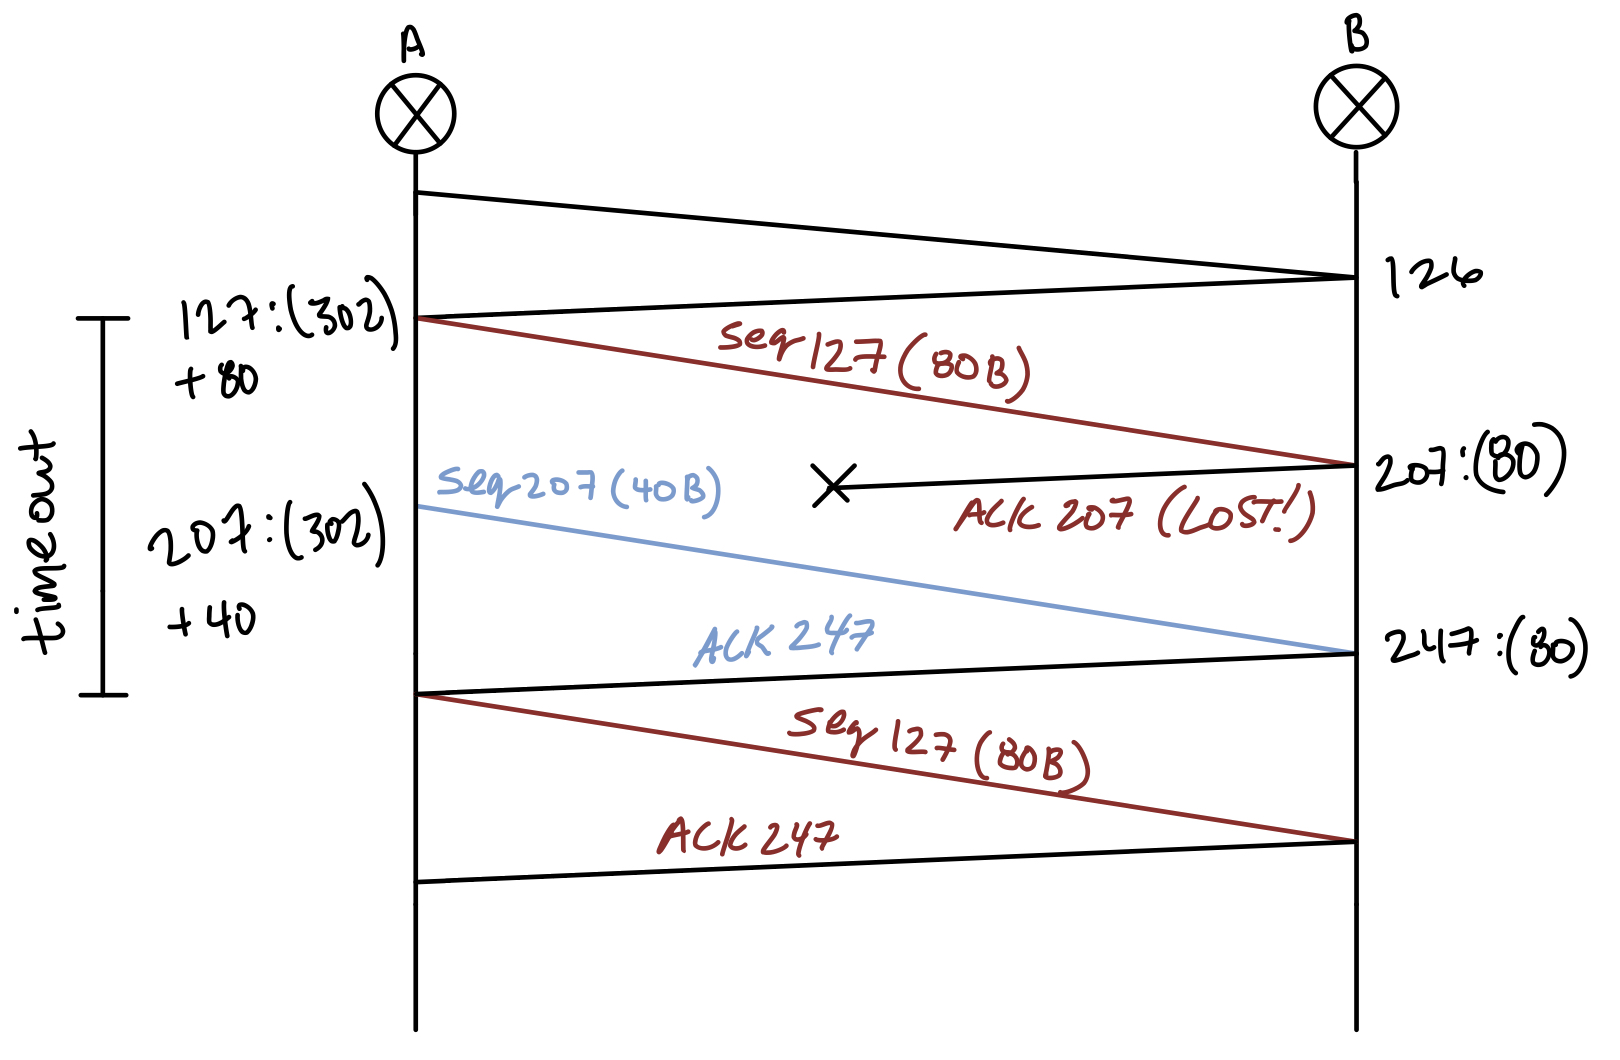
\includegraphics[width=0.65\textwidth]{HW3_P2.jpeg}
    \end{enumerate}
\large{\bfseries \item Problem 3}\par
    \begin{enumerate}
        \item Congestion Window\ =\ 16KB, no packet loss (slow-start state)
            \begin{table}[ht]
            \centering
            \begin{tabular}[t]{lccccc}
            \toprule
            & Initial & 1RTT & 2RTT & 3RTT & 4RTT\\ [1ex]
            \midrule
            \texttt{cwnd} & 1KB & 2KB & 4KB & 8KB & 16KB\\[1ex]
            \bottomrule
            \end{tabular}
            \end{table}\par
            $4RTT=4\times 100ms=\fcolorbox{blue}{white}{400ms}$
        \item Timeout at 16KB, no packet loss (congestion-avoidance state**)\par\vspace{0.25cm}
            \texttt{ssthresh}$\ =\frac{\texttt{cwnd}}{2}=\frac{16KB}{2}=$\ 8KB and \texttt{cwnd}\ =\ 1\par\vspace{0.25cm}
            \begin{table}[ht]
            \centering
            \begin{tabular}[t]{lcccccccccc}
            \toprule
            & Initial & 1RTT & 2RTT & 3RTT & 4RTT & 5RTT & 6RTT & 7RTT & 8RTT & 9RTT\\ [1ex]
            \midrule
            \texttt{cwnd} & 1KB & 2KB & 4KB & 8KB** & 9KB & 10KB & 11KB & 12KB & 13KB & 14KB\\[1ex]
            \bottomrule
            \end{tabular}
            \end{table}\par
            $9RTT=9\times 100ms=\fcolorbox{blue}{white}{900ms}$\vspace{0.5cm}
        \item Quadruple duplicate ACK event (fast-recovery state)\par\vspace{0.25cm}
            \texttt{ssthresh}$\ =\frac{\texttt{cwnd}}{2}=\frac{14KB}{2}=$\ 7KB and\\[0.5cm]\texttt{cwnd}$\ =\frac{\texttt{ssthresh}}{2}+\# \ Duplicates=3+4=7$KB\par\vspace{0.25cm}
            \begin{table}[ht]
            \centering
            \begin{tabular}[t]{lcccc}
            \toprule
            & Initial & 1RTT & 2RTT\\ [1ex]
            \midrule
            \texttt{cwnd} & 7KB & 8KB & 9KB\\[1ex]
            \bottomrule
            \end{tabular}
            \end{table}\par
            $2RTT=2\times 100ms=\fcolorbox{blue}{white}{200ms}$
    \end{enumerate}
\end{enumerate}
\end{document}
